%
% File acl2018.tex
%
%% Based on the style files for ACL-2017, with some changes, which were, in turn,
%% Based on the style files for ACL-2015, with some improvements
%%  taken from the NAACL-2016 style
%% Based on the style files for ACL-2014, which were, in turn,
%% based on ACL-2013, ACL-2012, ACL-2011, ACL-2010, ACL-IJCNLP-2009,
%% EACL-2009, IJCNLP-2008...
%% Based on the style files for EACL 2006 by 
%%e.agirre@ehu.es or Sergi.Balari@uab.es
%% and that of ACL 08 by Joakim Nivre and Noah Smith

\documentclass[11pt,letterpaper]{article}
\usepackage[hyperref]{acl2018}
\usepackage{CJKutf8}
\usepackage{times}
\usepackage{latexsym}
\usepackage{amsthm}
\usepackage{bbm}
\usepackage{mathtools,amssymb}
\usepackage{booktabs}
\usepackage{multirow}
\usepackage{multicol}
\usepackage{float}
\usepackage{array}
\usepackage{url}
\usepackage{algorithm}
\usepackage{algorithmicx}
\usepackage{algpseudocode}

\aclfinalcopy % Uncomment this line for the final submission
\def\aclpaperid{1279} %  Enter the acl Paper ID here

\setlength\titlebox{4cm}
% You can expand the titlebox if you need extra space
% to show all the authors. Please do not make the titlebox
% smaller than 5cm (the original size); we will check this
% in the camera-ready version and ask you to change it back.

\newcommand\BibTeX{B{\sc ib}\TeX}
% TODO Delete Finally.
\newcommand{\lzy}[1]{\textcolor{red}{\bf\small [#1 --note]}}
\newcommand*{\affaddr}[1]{#1} % No op here. Customize it for different styles.
\newcommand*{\affmark}[1][*]{\textsuperscript{#1}}
\renewcommand{\thefootnote}{\fnsymbol{footnote}}
\setcounter{footnote}{0}

\renewcommand{\algorithmicrequire}{\textbf{Input:}}
\renewcommand{\algorithmicensure}{\textbf{Output:}}

\title{11-747 Assignment 1: Text Classifier}
   
\author{Huiming Jin \\ \texttt{huimingj@andrew.cmu.edu}}
\date{}
 
\usepackage{scrextend}
\deffootnote[1.5em]{1.5em}{1em}{\thefootnotemark\space}
\renewcommand*{\thefootnote}{\roman{footnote}}

\begin{document}
\maketitle 
\begin{abstract}
    In this assignment, we implement multi-class text classifiers from scratch. 
    Besides the most basic CNN model, various deep neural architectures are 
    attempted, as well as several machine learning strategies for better 
    performance. With acceptable time and memory spending, the best model 
    achieves 86.8\% accuracy on the provided validation set. We also conduct a 
    series of experiments for analysis.
\end{abstract}

\section{Introduction}
    For this assignment, we are given simply pre-processed multi-class text
    classification task data. Each instance in the data is a sentence along with
    a single label that indicates the topic of the sentence.

    \begin{table}[htbp]
        \centering
        \small
        %\resizebox{\linewidth}{!}{
        \begin{tabular}{cp{4.2cm}}
            \toprule
                {\bf Label} & {\bf Sentence} \\
            \midrule
                Music       & The song was written by Madonna and produced by Benitez . \\
            \midrule
                Video games & The game was first released in North America , Europe and Australia in June 1991 , and in Japan the following month . \\
            \midrule
                Sports and recreation & The series went to seven games . \\
            \bottomrule
        \end{tabular}
        %}
        \caption{\label{tab:data-example} Sentence classification examples.}
    \end{table}

    Convolutional neural networks (CNN) has been widely used from computer 
    vision to natural language processing by showing its powerful capability.
    It utilizes filters and convolutional operations and can be considered as a
    kind of feature extraction, which can be then used by down-stream models.
    Comparing to Recurrent neural networks (RNN), CNN has better efficiency and
    can be easily stacked as very deep architectures. In this assignment, we 
    implement two kinds of CNN-based models: (1) TextCNN, and 
    (2) Deep Pyramid Convolutional Neural Networks (DPCNN).

    We implement the models using PyTorch\footnote{\url{https://github.com/oncebasun/nn4nlp19-hw1}}. 
    Besides model implementation, we also try some strategies to obtain better 
    performance, including using pre-trained embedding vectors, and model 
    ensemble et al. 
    
    We conduct experiments and try different hyper-parameter settings to select 
    the best setup for output. We also analyze the models to show the effects of
    different settings and data distribution.

    In the submission of this assignment, the predicted labels for the 
    validation set and the test set are listed in {\tt predict\_val.txt} and 
    {\tt predict\_test.txt} respectively, one label per line with the same order 
    as the original data.
    
\section{Methodology}
\subsection{TextCNN}
    \begin{figure}[htbp]
        \centering
        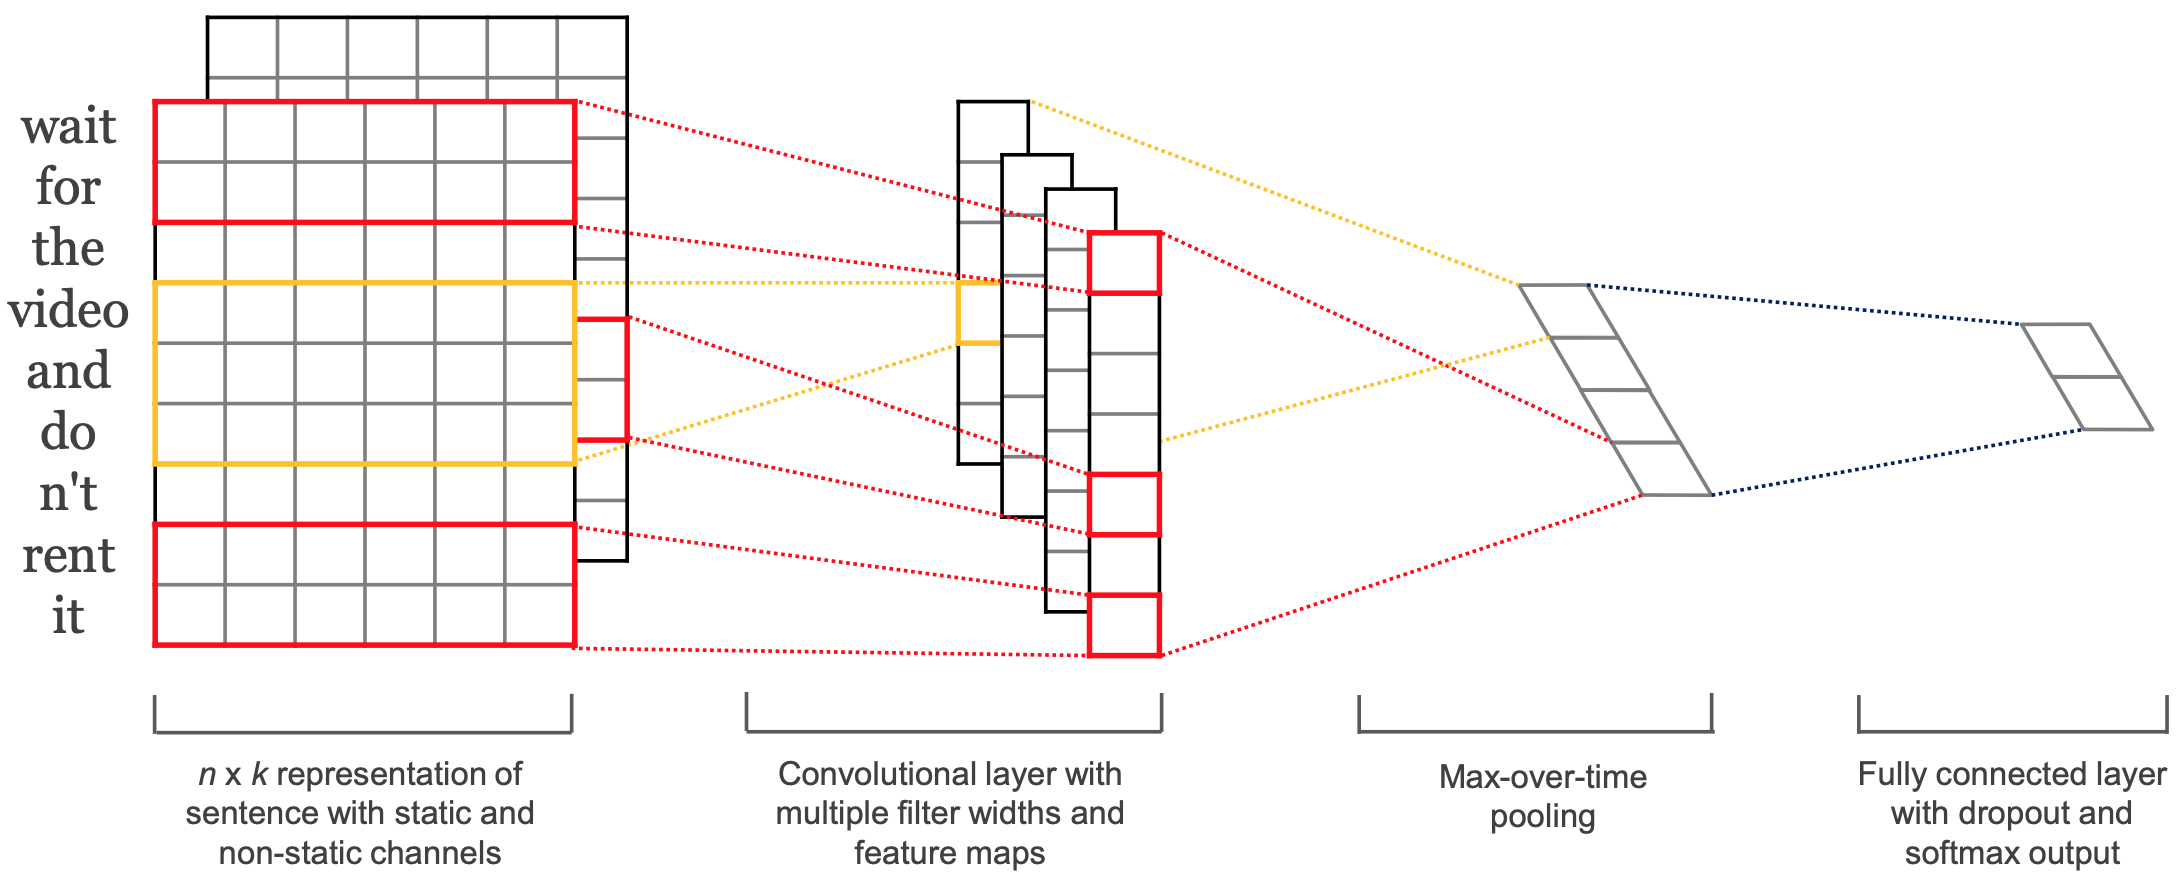
\includegraphics[width=\linewidth]{fig/1.png}  
        \caption{Architecture of TextCNN \cite{kim2014convolutional}.} 
        \label{fig:SSCNN}
    \end{figure}

    One model implemented in this assignment is single-layer TextCNN text 
    classifier proposed by \newcite{kim2014convolutional}, as shown in 
    Figure~\ref{fig:SSCNN}, which is a simple but powerful model. 

    Given a sentence $s=(x_1, \dots, x_n)$ where $x_i$ is the word in the
    sentence. Denote $\mathbf{x}_i \in \mathbb{R}^d$ as the vector 
    representation (word embedding) of $w_i$, where $d$ is the dimension of word 
    embedding. For convolutional operations, we need filters to be applied to 
    the sentence. Denote $C$ as the number of filters and each filter has 
    weights $\mathbf{w}_k\in\mathbb{R}^{hd}$, where $h$ is the filter width. The
    convolutional operation is defined as 
    \begin{align}
        z^{(k)}_i = \mathbf{w}_k \cdot \left[\mathbf{x}_i;\dots;\mathbf{x}_{i-h+1} \right] + b_k,
    \end{align} 
    where $\left[\mathbf{x}_i;\dots;\mathbf{x}_{i-h+1} \right]$ is the 
    concatenation of $\mathbf{x}_i\dots\mathbf{x}_{i-h+1}$, and it is followed 
    by non-linear activation function
    \begin{align}
        c^{(k)}_i = f(z^{(k)}_i).
    \end{align}
    After applying the filter from $i=1$ to $i=n-h+1$, we can attain the feature 
    map 
    \begin{align}
        \mathbf{c}^{(k)} = \left(c^{(k)}_1, c^{(k)}_2, \dots, c^{(k)}_{n-h+1}\right).
    \end{align}
    Then we apply max-pooling over the whole sentence to extract representative 
    feature for this filter
    \begin{align}
        \widehat{c}^{(k)} = \max\left\{\mathbf{c}^{(k)}\right\}.
    \end{align}
    Since we have multiple filters to extract multiple features respectively, we
    combine those features to a vector
    \begin{align}
        \widehat{\mathbf{c}} = \left(\widehat{c}^{(1)},\dots,\widehat{c}^{(C)}\right),
    \end{align}
    as the representation for the sentence. Then the sentence vector is passed
    to a fully connected layer followed by a softmax layer to obtain the 
    probabilities of labels:
    \begin{align}
        \mathbf{y} &= \mathbf{w}_{fc} \cdot \widehat{\mathbf{c}} + b_{fc} \\
        \mathbf{p} &= \text{softmax}(\mathbf{y}),
    \end{align}
    where $\mathbf{w}_{fc}$ and $b_{bf}$ are the weights and bias for the fully
    connected layer.

\subsection{Deep Pyramid CNN}
    As TextCNN only has one CNN layer which in theory can only extract very
    local features. However, as sentences are usually much longer than filter
    widths, and the long-distance dependencies may not be captured by the 
    filters, one intuitive idea is to use more CNN layers and local-pooling 
    layers to increase ranges that the features can be extracted, which has been 
    widely used in computer vision \cite{NIPS2012_4824,simonyan2014very,he2016deep,he2016identity}.

    \begin{figure}[htbp]
        \centering
        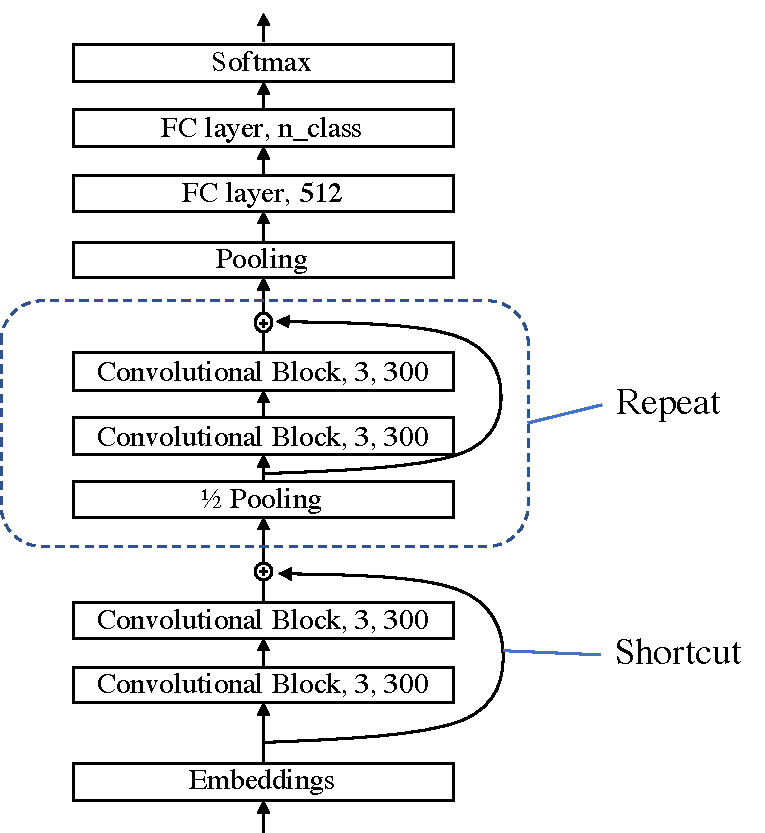
\includegraphics[width=\linewidth]{fig/3.pdf}  
        \caption{Architecture of DPCNN \cite{johnson2017deep}.} 
        \label{fig:DPCNN}
    \end{figure}

    Deep Pyramid CNN (DPCNN) is proposed by \newcite{johnson2017deep}, which uses 
    isometric CNN layers, which keeps the length of feature map same before and 
    after the CNN layer, to extract features, and 1/2 pooling layers with stride 
    step size 2 to reduce the length of feature maps by half. By using this 
    setup, DPCNN can efficiently capture long-distance features without too many 
    learnable parameters. Fig. \ref{fig:ICNN} illustrates the design of 
    isometric CNN and 1/2 pooling layers. 

    \begin{figure}[htbp]
        \centering
        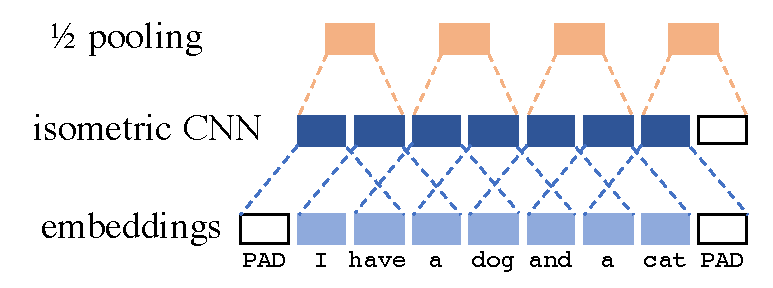
\includegraphics[width=\linewidth]{fig/2.pdf}  
        \caption{Isometric CNN and 1/2 pooling layers \cite{johnson2017deep}.} 
        \label{fig:ICNN}
    \end{figure}

    \paragraph{Shortcut connections.} As the networks become much deeper, many
    previous works have shown that deep networks are much harder to optimize.
    To overcome this problem, \newcite{he2016deep} introduce shortcut connection
    in ResNet, by which the input of convolutional blocks are added to the 
    output:
    \begin{align}
        \mathbf{z} = \mathbf{x} + f(\mathbf{x}).
    \end{align}

    \paragraph{Fixed feature map number.} Although many computer vision models
    increase the number of feature maps for deeper CNN layers, it may not so
    feasible for text classification, since the dimension of input word 
    embeddings is usually large enough while images usually only have three 
    input channels, thus increasing feature map number causes increased 
    computation time but does not improve the accuracy significantly. Moreover,
    using the fixed feature map number makes shortcut connections easier because 
    we do not need additional operations for dimension matching. 

    Fig. \ref{fig:DPCNN} shows the Architecture of DPCNN. In our implementation,
    the filter window size is 3 and the feature map number is 300. Each 
    convolutional layer and fully connected layer is followed 
    batch-normalization layer ReLU activation function.

\section{Additional Strategies}
    Besides exploring different neural network architectures, we also try some
    additional strategies to help our networks to perform better.

\subsection{Regularization}
    As deep neural networks are easy to overfit the training data, we use 
    regularization strategy to tackle this problem.

    %TODO:
    \paragraph{Dropout.} We apply dropout \cite{hinton2012improving} operation 
    before the first fully connected layer. In the training phase, dropout 
    operation randomly set some hidden unit (values of feature vector) to zero 
    by a pre-defined probability $p$. In the evaluation phase, the feature 
    vector is scaled by the factor $p$.

    \paragraph{L2-Regularization.} We also apply L2 regularization which adds 
    the sum of weight L2-norms scaled by pre-defined $\lambda$ to the loss in 
    optimizing:
    \begin{align}
        loss' = loss + \lambda\sum||\mathbf{w}||_2.
    \end{align}

\subsection{Pre-trained word embeddings}
    We use real-valued vectors (embeddings) to represent the words as inputs. 
    Word embeddings are expected to encode the semantic meanings of individual 
    words. However, since the training data for supervised tasks are usually 
    insufficient, the word embeddings learned in those tasks may not in good
    quality. For better word representations, we use word embeddings learned by 
    unsupervised tasks in which the training corpora contain billions of words.
    Specifically, we use the word embeddings pre-trained by fastText 
    \cite{mikolov2018advances}. The randomly initialized word embeddings of the 
    words that present in the pre-training corpus are replaced by pre-trained
    word vectors.

\subsection{Ensemble}
    Different model designs, settings, and initializations may affect the
    models' prediction of particular instances. To make our model more robust, 
    we could train a series of different models and combine their predictions
    by weighted addition. Specifically, for a sentence input $s$, assume that
    we have $M$ models and each model $m_i$ will predict a label $y_i$. The 
    ensemble prediction 
    \begin{align}
        \hat{y} = \underset{y}{\mathrm{argmax}}\left\{score(y)=\sum_i\alpha_i\mathbb{I}[y_i=y]\right\},
    \end{align}
    where $\alpha_i$ is the weight for model $m_i$, which is simply set to the 
    corresponding accuracy on the dev set in our implementation.

\section{Experiments}
\subsection{Dataset and Experimental Setup}
    We conduct experiments on the provided sentence topic classification
    dataset. The provided data is already tokenized. In our experiments, we
    change the words into lower cases to reduce vocabulary sparsity. 
    Additionally, we change the wrongly spelled label ``darama'' in the 
    validation to ``drama''.

    We use Adam \cite{kingma2014adam} as the optimization method with 
    cross-entropy loss. In training, we use early stopping on the validation set 
    and shuffled mini-batches that pads sentences to the same length.

    For all models, we set the learning rate as $10^{-4}$ and the mini-batch 
    size as 512 which are relatively good in all experiments. The kernel sizes 
    of TextCNN are 3,4,5, and the kernel size of DPCNN is 3. Dropout 
    probability is set to $0.5$. For pre-trained word embeddings, we use the 
    300-dimensional vectors trained by fastText on Common 
    Crawl\footnote{\url{https://fasttext.cc/docs/en/english-vectors.html}}, 
    which contains 600B tokens and is not fixed in training. We also rescale 
    (clip) the L2-norm of gradients to $1$ if it is greater than $1$ to avoid 
    unstable back-propagation. For all individual models, we select the best 
    other corresponding hyper-parameters respectively, including L2 penalty 
    coefficients, in reporting the accuracies.

\subsection{Results and Discussion}
\subsubsection{Overall Results}
    Model variations are investigated to show the effect of different model 
    complexities. Table.~\ref{tab:primary} shows the experimental results on the
    dev set, where the number following ``TextCNN-'' represents the number of 
    filters for each kernel size. The number after ``DPCNN-'' represents how 
    many 1/2~pooling-CNN-CNN block (the dashed box in Fig.~\ref{fig:DPCNN}) 
    stacks in the DPCNN model. The ensemble model is the combination of all
    TextCNN and DPCNN models.

    \begin{table}[htbp]
        \centering
        %\small
        %\resizebox{\linewidth}{!}{
        \begin{tabular}{ccc}
            \toprule
                {\bf Method}    & {\bf Time per epoch}  & {\bf Acc.(\%)} \\
            \midrule
                TextCNN-100     & 14s                   & 85.5 \\
                TextCNN-200     & 20s                   & 86.1 \\
                TextCNN-300     & 27s                   & 86.2 \\
                DPCNN-1         & 22s                   & 85.4 \\
                DPCNN-2         & 25s                   & 85.5 \\
                DPCNN-3         & 27s                   & 83.8 \\
                Ensemble        & --                    & {\bf 86.8} \\
            \bottomrule
        \end{tabular}
        %}
        \caption{\label{tab:primary} Test results on dev set.}
    \end{table}

    We could observe that both TextCNN and DPCNN can achieve promising 
    evaluation, but deeper models such as DPCNN do not necessarily promise
    better performance as the training time increases. However, the TextCNN
    model can perform better with more filter numbers.

    One possible reason for this phenomenon is the nature of this task. TextCNN
    tends to capture local features while DPCNN is good at capturing 
    long-distance dependencies. However, local features might be already enough 
    for the sentence topic classification task. If we look at the data, we could
    find that the topic of the sentences could be inferred by some 
    representative keywords or phrases in many cases. For example, words like 
    ``song'' and ``band'' are very typical of the topic ``Music''. In this 
    scenario, long-distance features are not so important as in some other tasks 
    such as sentiment analysis and humor detection. Therefore, since deep models 
    with more learnable parameters are also easy to overfit the training data, 
    DPCNN performs worse with more layers. For other tasks as mentioned above, 
    we could expect DPCNN to achieve better results than TextCNN.

    As our expectation, the ensemble model outperforms other models since it is
    more robust. Because TextCNN and DPCNN are similar models, the improvement
    attained by the ensemble model is not really significant. If we developed
    more diverse models and using better integration methods, we could expect 
    better performance of the ensemble model, as different models could capture 
    different kinds of features.


    \begin{table*}[htbp]
        \centering
        %\small
        \resizebox{\linewidth}{!}{
        \begin{tabular}{cccc}
            \toprule
                {\bf Label}                 & {\bf Train Freq.} & {\bf Acc.}    & {\bf Common error}  \\
            \midrule
                Social sciences and societ  & 8.06\%            & 83.93\%       & History           \\
                Sports and recreation       & 12.31\%           & 91.57\%       & Media and drama   \\
                Natural sciences            & 11.70\%           & 100.00\%      & --                \\
                Language and literature     & 2.93\%            & 77.78\%       & Sports and recreation, Video games\\
                Geography and places        & 4.82\%            & 77.78\%       & Art and architecture \\
                Music                       & 13.30\%           & 94.03\%       & Social sciences and society \\
                Media and drama             & 10.01\%           & 91.75\%       & Social sciences and society, Natural sciences \\
                Art and architecture        & 4.02\%            & 61.54\%       & History \\
                Warfare                     & 10.29\%           & 92.41\%       & Social sciences and society \\
                Engineering and technology  & 7.23\%            & 84.75\%       & Art and architecture \\
                Video games                 & 4.67\%            & 100.00\%      & -- \\
                History                     & 7.26\%            & 62.79\%       & Warfare \\
            \bottomrule
        \end{tabular}
        }
        \caption{\label{tab:labels} The label frequencies in the train set and corresponding accuracies on the dev set. The most common error cases are the labels that mostly wrongly predicted on the dev set.}
    \end{table*}

\subsubsection{Impact of Different Settings}
    We conduct a series of experiments to analyze how different hyper-parameters
    affect the performance of neural networks. 

    \begin{table}[htbp]
        \centering
        %\small
        \resizebox{\linewidth}{!}{
        \begin{tabular}{ccc}
            \toprule
                {\bf Word embeddings}   & {\bf TextCNN-300} & {\bf DPCNN-2} \\
            \midrule
                Random                  & 77.9              & 73.7          \\
                wiki-news-300d-1M       & 82.6              & 84.1          \\
                crawl-300d-2M           & {\bf 86.2}        & {\bf 85.5}    \\
            \bottomrule
        \end{tabular}
        }
        \caption{\label{tab:wordvec} Accuracies of TextCNN-300 and DPCNN-2 with different word embedding initializations.}
    \end{table}

    \paragraph{Pre-trained word embeddings.} We also attempt to use different
    pre-trained word embeddings as they learn different semantics from different
    corpora. Besides the vectors trained on Common Crawl, we also try the 
    vectors trained on Wikipedia 2017, UMBC webbase corpus and statmt.org news 
    dataset (16B tokens) by fastText\footnote{\url{https://fasttext.cc/docs/en/english-vectors.html}},
    and randomly initialized word embeddings.

    As shown in Table \ref{tab:wordvec}, word embedding initialization crucially 
    influences the final results. The vecotrs learned from larger dataset 
    (crawl-300d-2M) greatly improves the accuracy comparing to smaller dataset 
    (wiki-news-300d-1M) and random initialization. 

    \begin{table}[htbp]
        \centering
        %\small
        %\resizebox{\linewidth}{!}{
        \begin{tabular}{ccc}
            \toprule
                {\bf $\lambda$} & {\bf TextCNN-300} & {\bf DPCNN-2} \\
            \midrule
                $0$             & 81.6              & 85.2       \\
                $10^{-5}$       & 84.6              & 84.3       \\
                $10^{-4}$       & {\bf 86.2}        & {\bf 85.5} \\
                $10^{-3}$       & 84.6              & 83.7       \\
                $10^{-2}$       & 85.6              & 84.8       \\
                $10^{-1}$       & 70.3              & 84.0       \\
            \bottomrule
        \end{tabular}
        %}
        \caption{\label{tab:l2} Accuracies of TextCNN-300 and DPCNN-2 with different $\lambda$.}
    \end{table}


    \paragraph{L2 regularization.} The choice of the L2-regularization 
    coefficient $\lambda$ is crucial since it balances the capability of the 
    model and prevents overfitting. We show the performances of TextCNN-300 and 
    DPCNN-2 with different L2-regularization coefficients in Table \ref{tab:l2}.
   
    In general, both too large and too small $\lambda$ values damage the 
    performance, though it is not so notable for DPCNN-2. With greater 
    $\lambda$, the accuracy of TextCNN-300 decreases greatly, as TextCNN is not 
    so complex as DPCNN, and greater $\lambda$ tends to cause underfitting.

\subsubsection{Error Analysis}

\begin{table}[htbp]
    \centering
    %\small
    \resizebox{\linewidth}{!}{
    \begin{tabular}{cccc}
        \toprule
            {\bf Word frequency}    & {\bf Train}   & {\bf Correct} & {\bf Incorrect} \\
        \midrule
            $[0,1)$                 & --            & 3.60\%        & 3.22\%    \\
            $[1,2)$                 & 41.73\%       & 1.32\%        & 1.11\%    \\
            $[2,5)$                 & 25.32\%       & 2.42\%        & 1.88\%    \\
            $[5,20)$                & 19.75\%       & 9.05\%        & 5.76\%    \\
            $[20,10^2)$             & 8.72\%        & 19.54\%       & 14.86\%   \\
            $[10^2,10^3)$           & 3.93\%        & 47.19\%       & 39.69\%   \\
            $[10^3,10^4)$           & 0.51\%        & 15.62\%       & 28.38\%   \\
            $[10^4,10^5)$           & 0.03\%        & 1.05\%        & 4.21\%    \\
            $\geq 10^5$             & 0.01\%        & 0.21\%        & 0.89\%    \\
        \bottomrule
    \end{tabular}
    }
    \caption{\label{tab:wordfreq} Word frequency distributions among the train set, correct dev set, and incorrect dev set.}
\end{table}

    \paragraph{Word frequencies.} The performance of models is closely related 
    to the data. One typical factor that affects the prediction results is the 
    distribution of words. Table \ref{tab:wordfreq} shows the distributions of 
    word frequency (the number of times that the word appears in the train set) 
    in the train set, the correctly classified sentences in the dev set, and 
    the incorrectly classified sentences in the dev set. The classification
    results are from the ensemble model.

    We could observe that most words in the training data are low-frequency 
    words, and low-frequency words hurt the efficacy of the classification 
    models since the network will be less activated by them. On the other hand, 
    words with extremely high frequencies may be too common that they are not 
    informative, such as ``the'', ``and'', and punctuations. Compared to the 
    correctly classified sentences, wrongly classified sentences also contain 
    more high-frequency words and less medium-frequency words, which may confuse
    the models and lead to error.

    \paragraph{Label distribution.} We also investigate the effect of label 
    distributions. Table \ref{tab:labels} shows the statistics of labels on 
    the train set and respective accuracies on the dev set as well as the most
    common error cases. In general, the more training samples the labels have in 
    the train set, the higher accuracies we can obtain. Meanwhile, if two topics
    are closely related, then it will confuse the model and make it difficult to
    predict, such as {\it History} and {\it Warfare}, {\it Sports and recreation}
    and many other topics.
    
\section{Conclusion}
    In this assignment, we implemented TextCNN and DPCNN with different specific
    settings using PyTorch and conducted a series of experiments to analyze the 
    results. The best ensemble achieves 86.8\% accuracy on the provided 
    validation set.
 
\vspace{1em} 
% include your own bib file like this:
%\bibliographystyle{acl}
%\bibliography{acl2018}
\bibliography{acl2018}
\bibliographystyle{acl_natbib}
 
\appendix

\end{document}
